\section{Eletrônica Embarcada}
\label{EEA}


\begin{table}[ht!]

	\begin{tabular}{r l|l p{12cm} }
		
		\textcolor{gray}{Especificação} &&& 	{Eletrônica Embarcada à prova d'água,
		Umbilical e Sistema eletrônico de superfície}\\
		\textcolor{gray}{Data} &&& 				{14/06/2014}\\
        \textcolor{gray}{Beneficiado} &&&		{Ground Truth Robotics GmbH} \\
        \textcolor{gray}{CNPJ} &&& 				{Internacional} \\
        \textcolor{gray}{Número Nota} &&& 		{251-A-2014} \\
		\textcolor{gray}{Quantidade} &&& 		{1} \\
		\textcolor{gray}{Valor} &&& 			{R\$887.263,26} \\
		\textcolor{gray}{Data Sheet} &&& 		{-} \\

		\textcolor{gray}{Função no projeto} &&& {Produto final, projeto e execução, da
		eletrônica embarcada à prova d'água e sistema de superfície.}
		\\
		\textcolor{gray}{Razão da Escolha} &&& {Parceira no desenvolvimento de robôs
		(DFKI).}
	\end{tabular}
\end{table}

\newpage

\subsection{Foto do Material}
\begin{figure}[H]
 \centering
 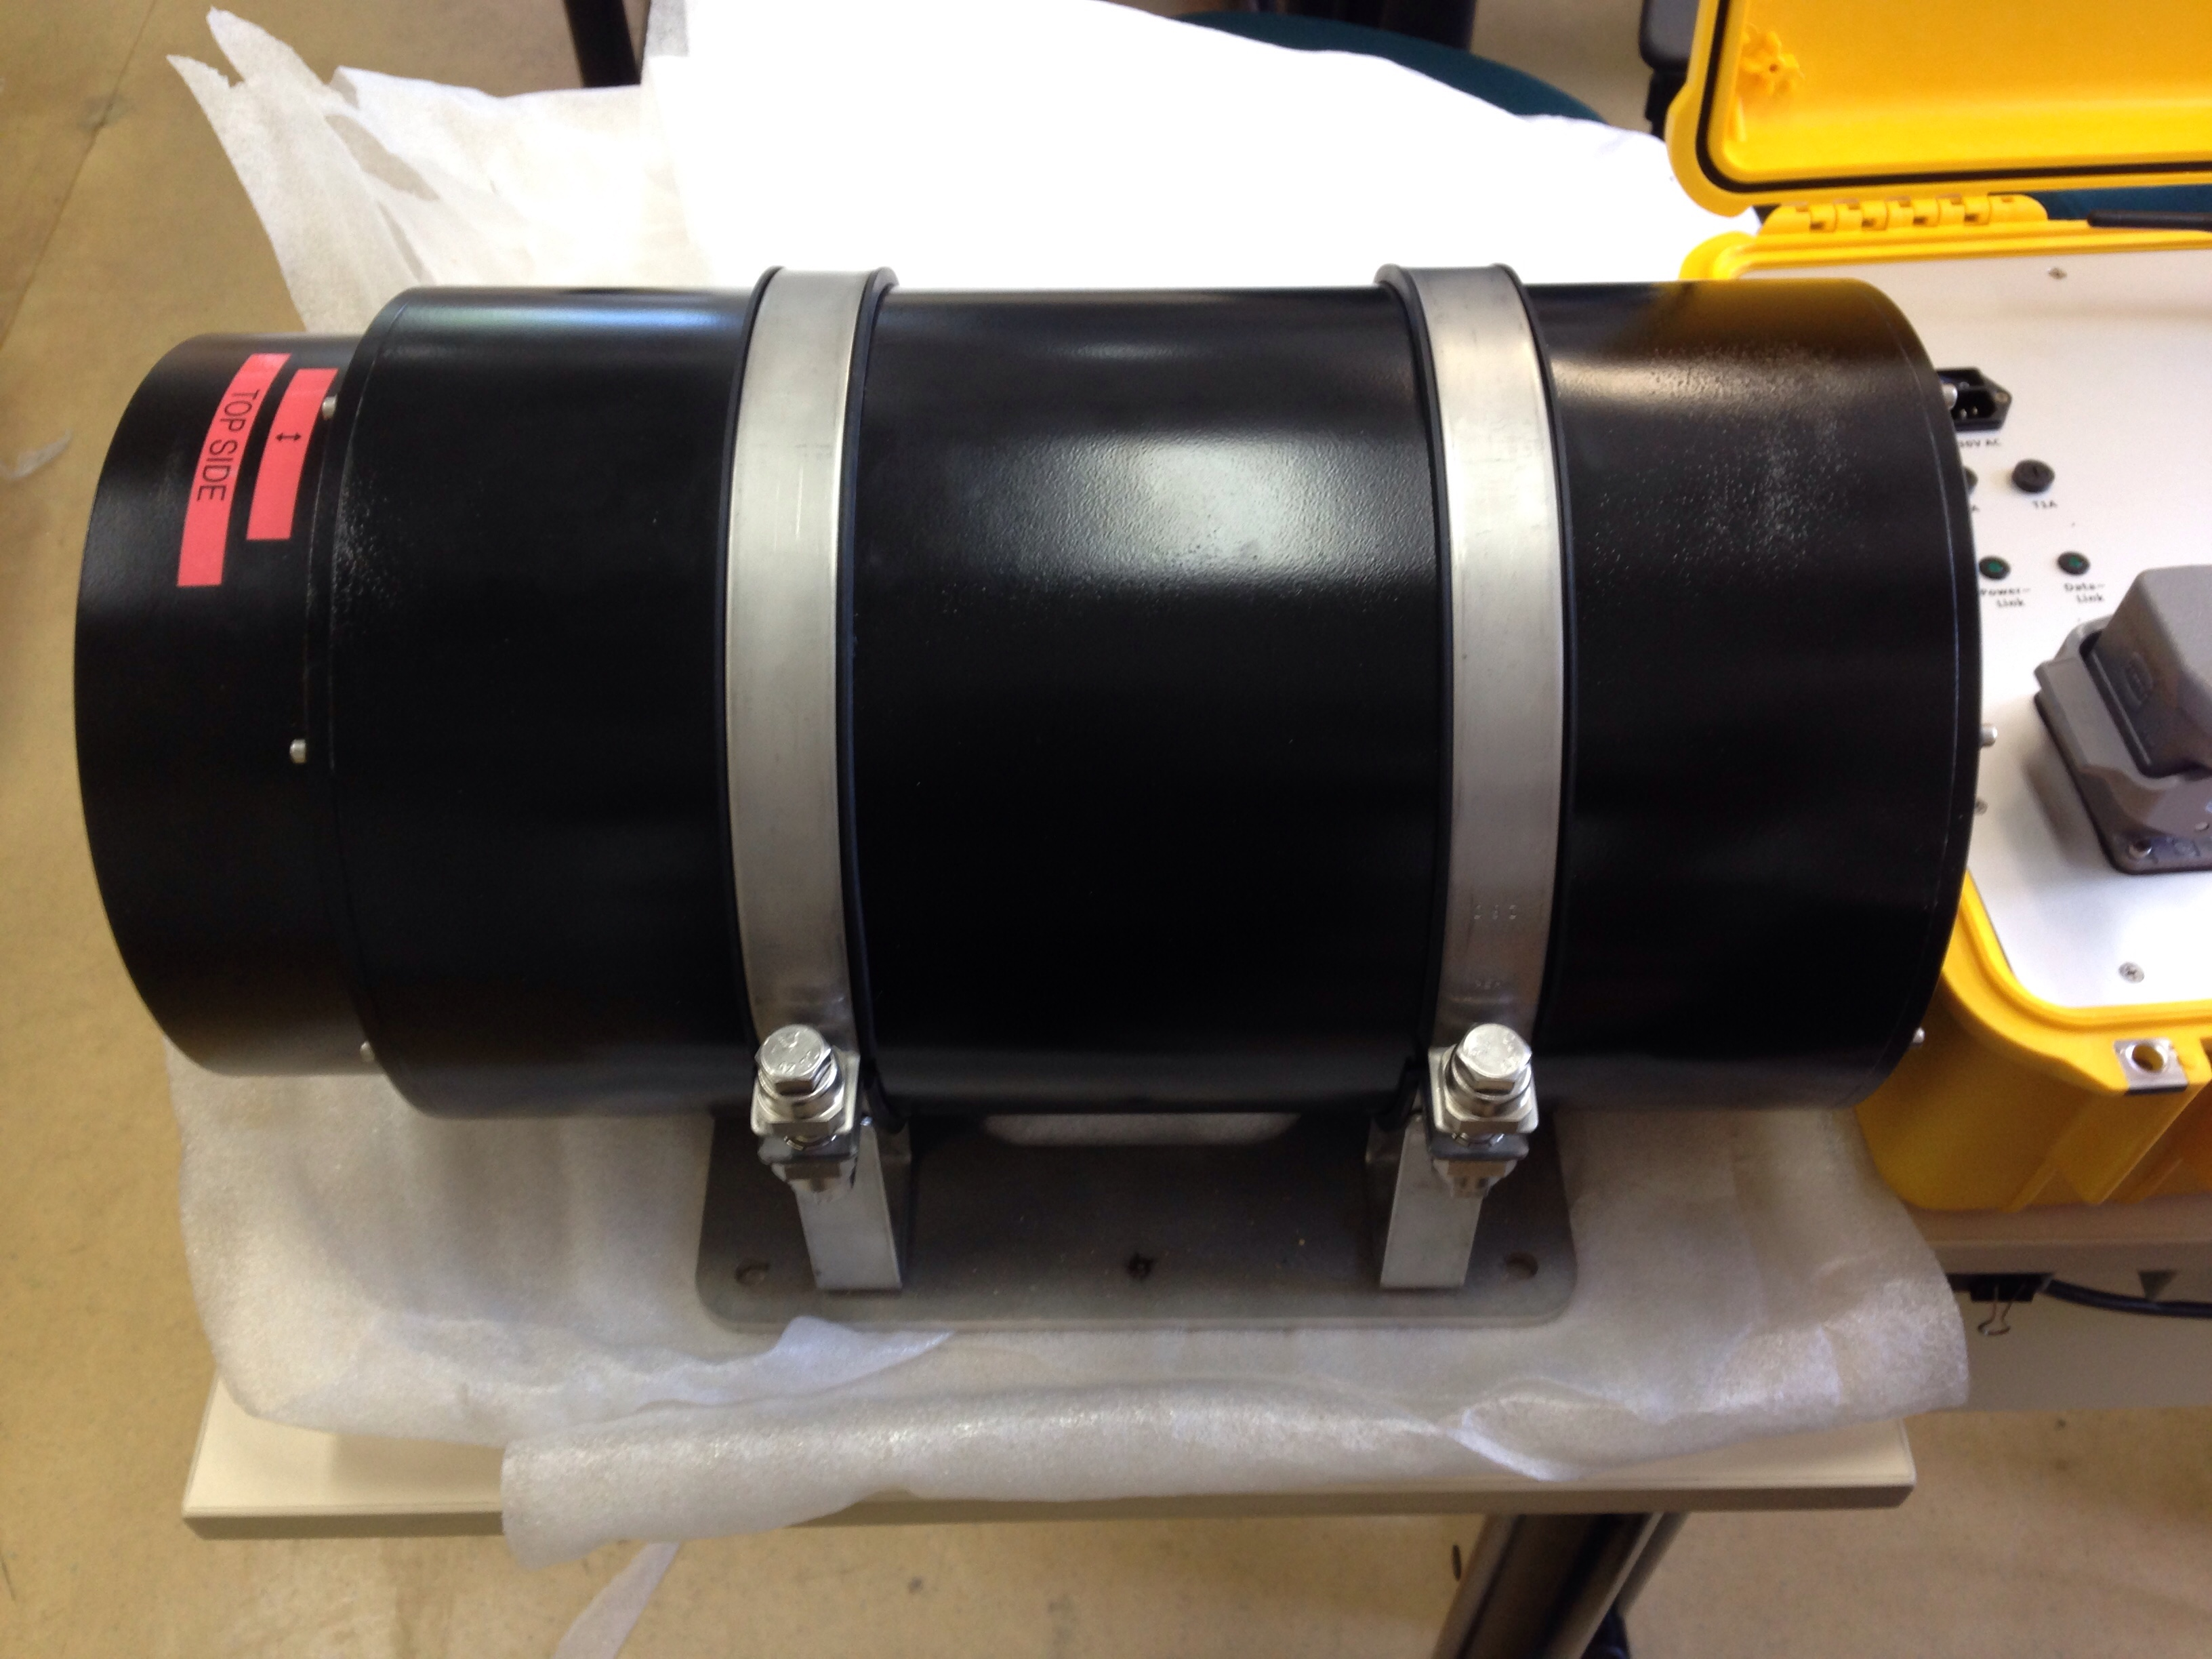
\includegraphics[width=1\columnwidth]{EEA/foto1.jpg}
 \caption{Housing da Eletrônica à prova d'água}
\end{figure}

\subsection{Foto do Material 2}
\begin{figure}[H]
 \centering
 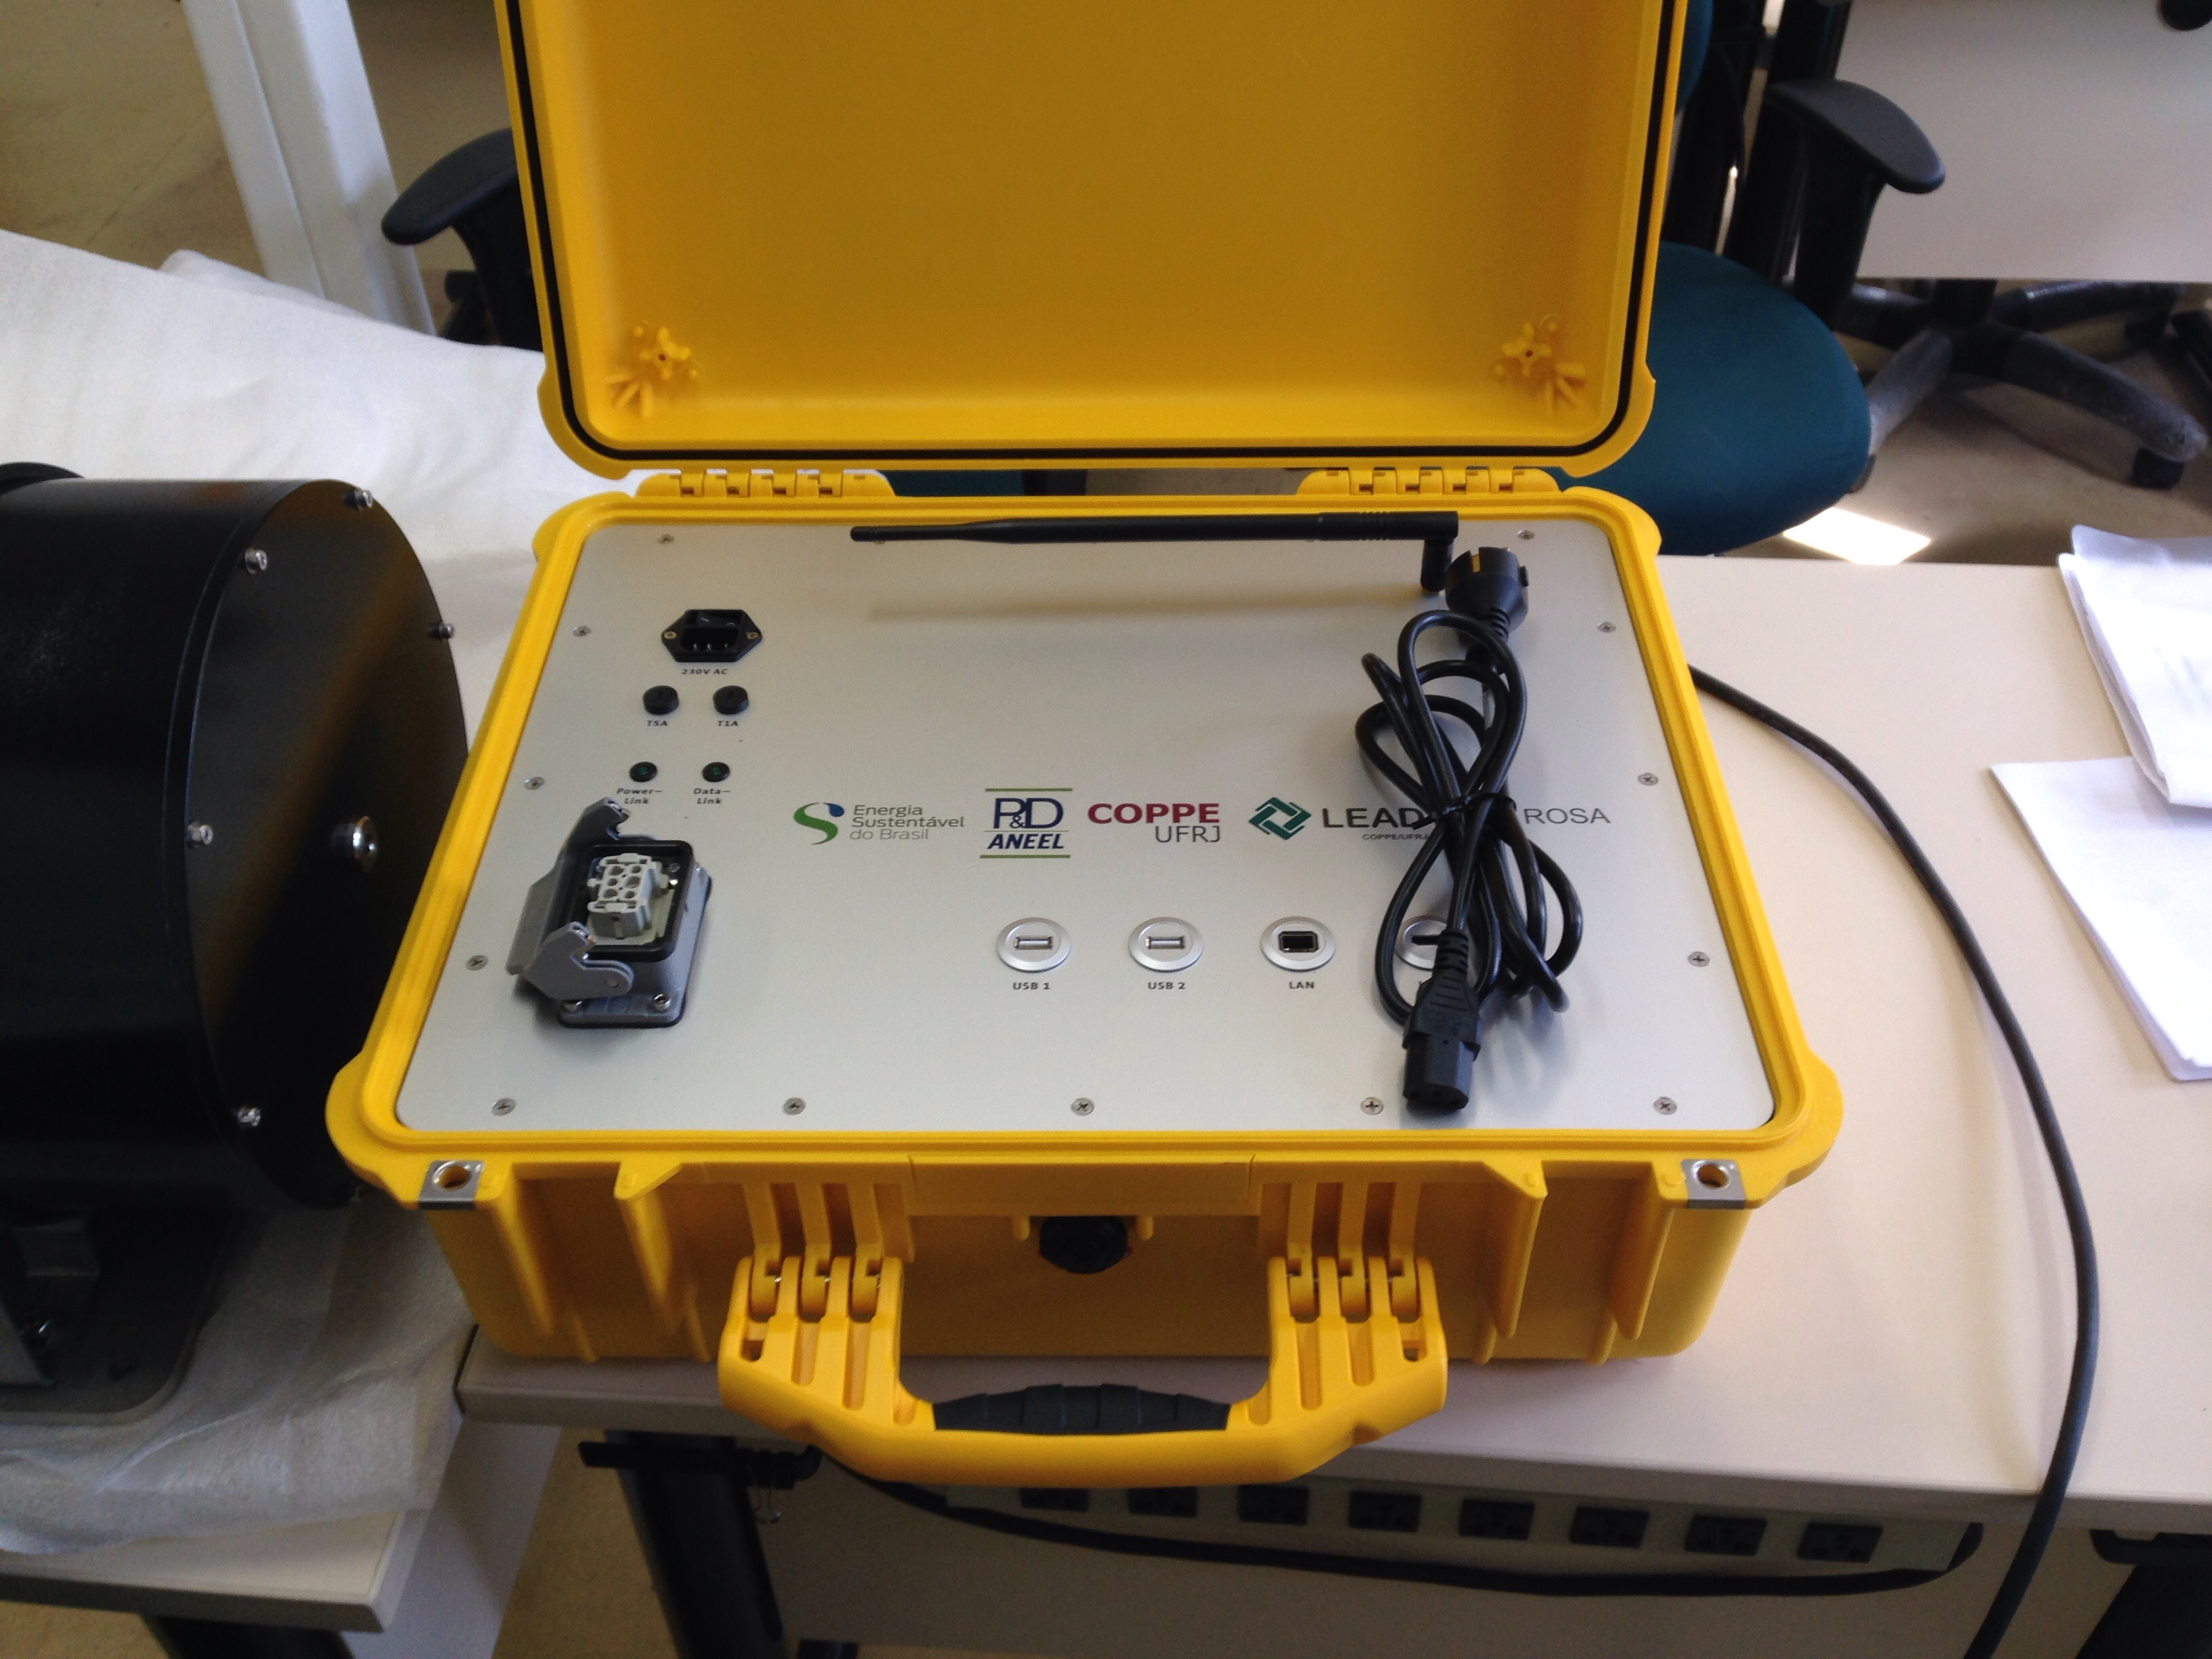
\includegraphics[width=1\columnwidth]{EEA/foto2.jpg}
 \caption{Pelican case da eletrônica de superfície}
\end{figure}

\subsection{Nota Fiscal}
\begin{figure}[H]
 \centering
 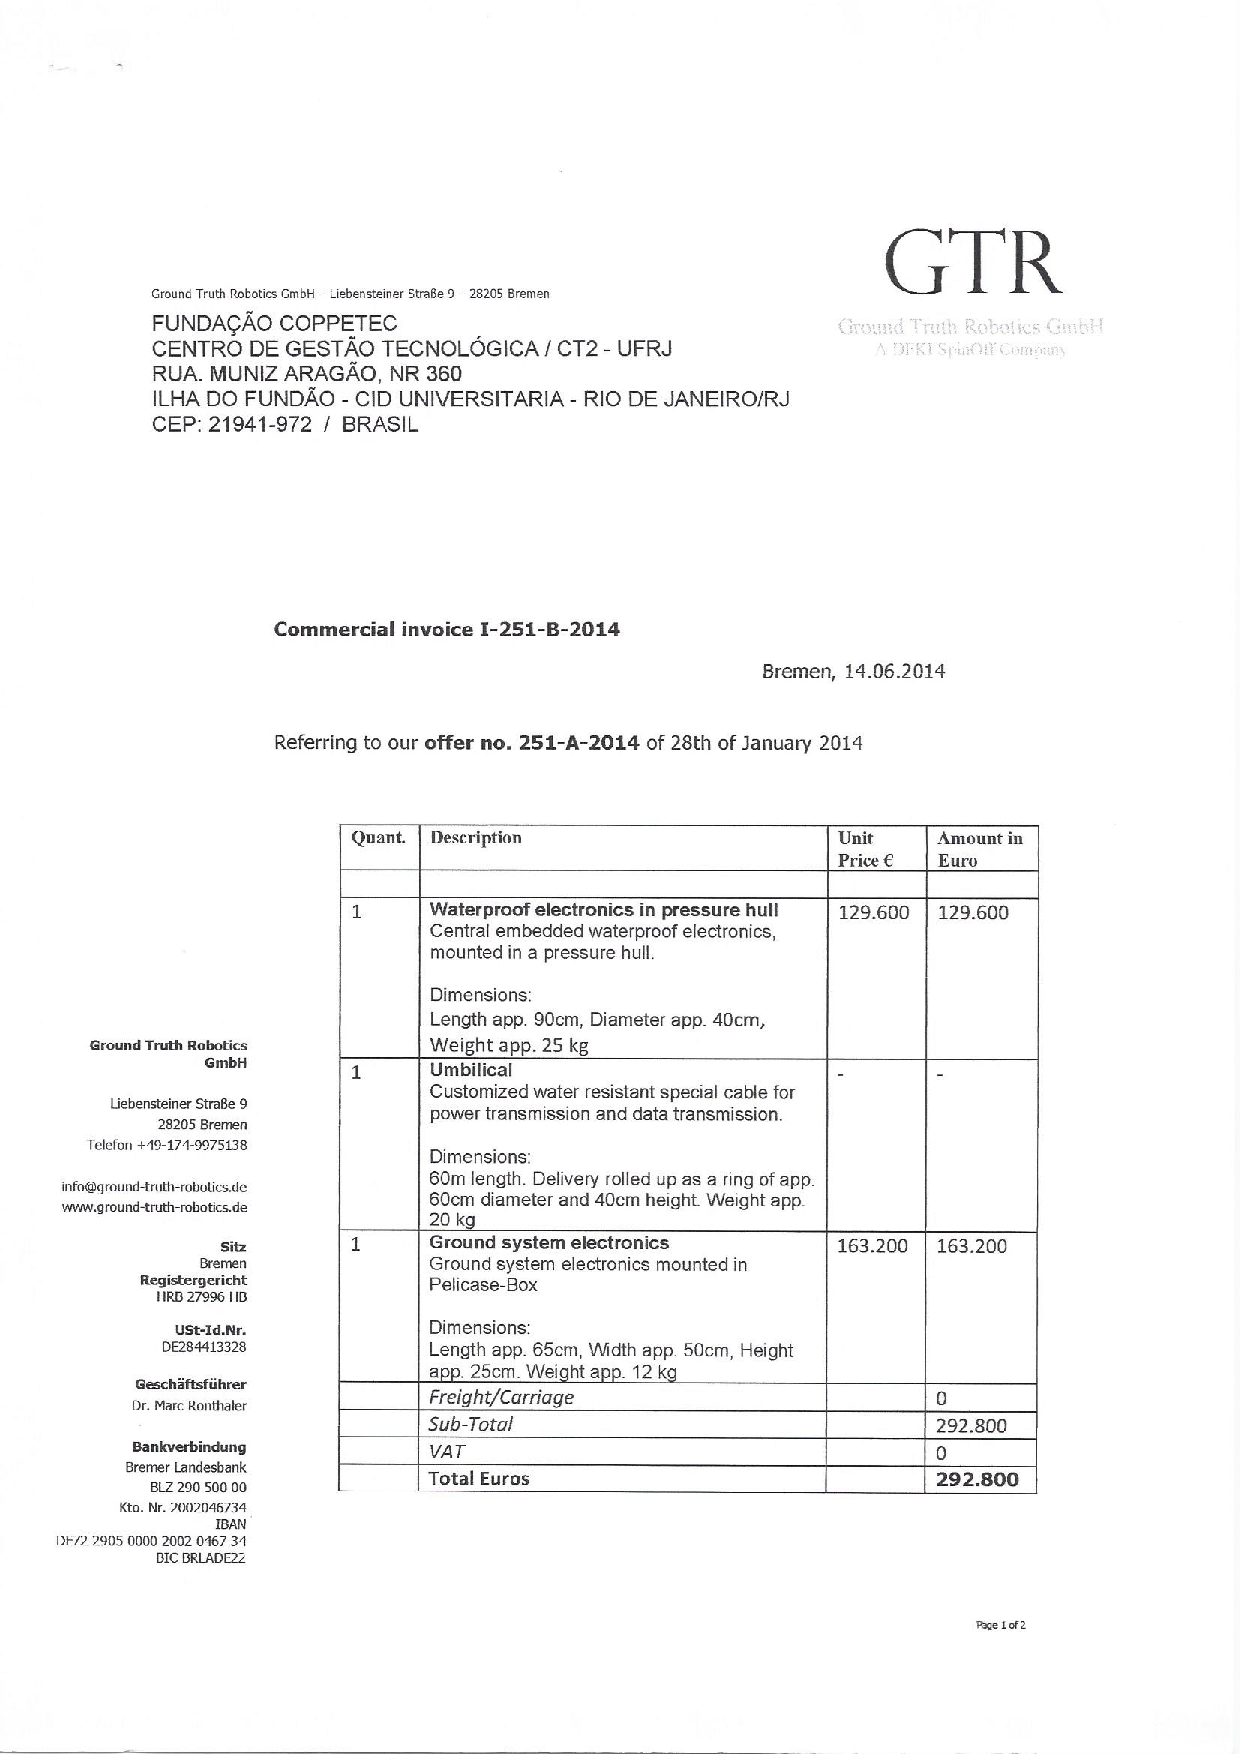
\includegraphics[width=0.9\columnwidth]{EEA/nota_gtr.pdf}
 \caption{Nota fiscal da eletrônica embarcada}
\end{figure}


